\documentclass[12pt]{article}
\usepackage{amsmath}
\usepackage{amssymb}
\usepackage{tikz}
\usetikzlibrary{shapes}
\usepackage{color}
\usepackage[utf8]{inputenc}

\begin{document}

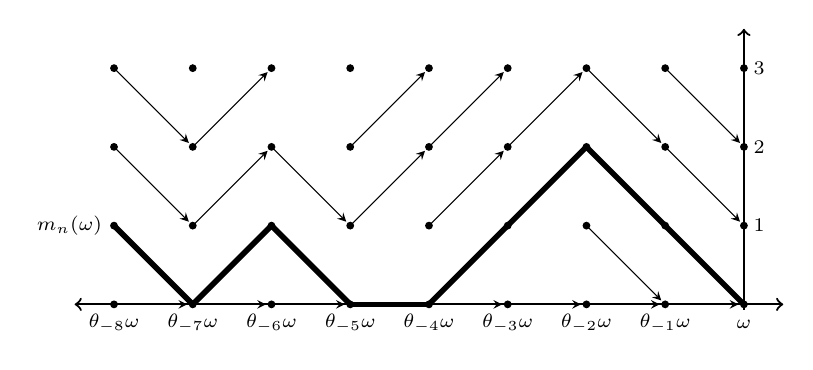
\begin{tikzpicture}
    \foreach \x in {-8,...,0}{
        \ifnum\x<0
            \coordinate[label=below:\scriptsize$\theta_{\x} \omega$] (\x-0) at (\x, 0);
        \fi
        \node[shape=circle,fill=black,scale=0.3] (\x-0) at (\x, 0){};
        \foreach \y in {1,...,3}{
            \ifnum\x=0
                \coordinate[label=right:\scriptsize$\y$] (0-\y) at (0, \y);
            \fi
            \node[shape=circle,fill=black,scale=0.3] (\x-\y) at (\x, \y){};
        }
    }

    \tikzstyle{thickline}=[line width=0.7mm]

    \draw[thick, <->] (-8.5, 0) -- (0.5, 0);
    \draw[thick, ->] (0, -2pt) node[anchor=north]{\scriptsize$\omega$} -- (0, 3.5);
    \draw[thickline] (-8, 1) node[anchor=east]{\scriptsize$m_n(\omega)$} -- (-7, 0);
    \draw[thickline] (-7, 0) -- (-6, 1);
    \draw[thickline] (-6, 1) -- (-5, 0);
    \draw[thickline] (-5, 0) -- (-4, 0);
    \draw[thickline] (-4, 0) -- (-3, 1);
    \draw[thickline] (-3, 1) -- (-2, 2);
    \draw[thickline] (-2, 2) -- (-1, 1);
    \draw[thickline] (-1, 1) -- (0, 0);

    \draw[-stealth, shorten >=2pt] (-8, 2) -- (-7, 1);
    \draw[-stealth, shorten >=2pt] (-7, 1) -- (-6, 2);
    \draw[-stealth, shorten >=2pt] (-6, 2) -- (-5, 1);
    \draw[-stealth, shorten >=2pt] (-5, 1) -- (-4, 2);
    \draw[-stealth, shorten >=2pt] (-4, 2) -- (-3, 3);
    \draw[-stealth, shorten >=2pt] (-2, 3) -- (-1, 2);
    \draw[-stealth, shorten >=2pt] (-1, 2) -- (0, 1);

    \draw[-stealth, shorten >=2pt] (-8, 3) -- (-7, 2);
    \draw[-stealth, shorten >=2pt] (-7, 2) -- (-6, 3);
    \draw[-stealth, shorten >=2pt] (-5, 2) -- (-4, 3);
    \draw[-stealth, shorten >=2pt] (-1, 3) -- (0, 2);

    \draw[-stealth, shorten >=2pt] (-4, 1) -- (-3, 2);
    \draw[-stealth, shorten >=2pt] (-3, 2) -- (-2, 3);
    \draw[-stealth, shorten >=2pt] (-2, 1) -- (-1, 0);

    \draw[-stealth, shorten >=2pt] (-8, 0) -- (-7, 0);
    \draw[-stealth, shorten >=2pt] (-7, 0) -- (-6, 0);
    \draw[-stealth, shorten >=2pt] (-6, 0) -- (-5, 0);
    \draw[-stealth, shorten >=2pt] (-4, 0) -- (-3, 0);
    \draw[-stealth, shorten >=2pt] (-3, 0) -- (-2, 0);
    \draw[-stealth, shorten >=2pt] (-2, 0) -- (-1, 0);
    \draw[-stealth, shorten >=2pt] (-1, 0) -- (0, 0);
\end{tikzpicture}

\end{document}